% PrototypeDevelopmentLifecycle.tex
\subsection{Lifecycle}
This section provides an overview of the Prototype Develop ment Lifecycle.

% Include a flowchart
% \begin{figure}[H]
%     \centering
%     \scalebox{0.8}{ % Scale to 80% of original size
%         % try generating flowcharts as svg in Claude 
% and edit with inkscape instead of this.
% but claude did generate this one so might 
% be useful too but you can't easily make
% small repairs in inkscape


% CNN Transfer Learning Flowchart - Compact Multi-Column Layout
% \begin{figure}[htbp]

\centering
\resizebox{\textwidth}{!}{ % Scale to fit width while maintaining aspect ratio
\begin{tikzpicture}[node distance=0.8cm and 1.5cm, auto]
    % Define a smaller block style
    \tikzset{
      block/.style = {rectangle, draw, fill=blue!20, 
                      text width=7em, text centered, rounded corners, minimum height=1.8em, font=\small},
    }
    
    % Brazilian model training - Column 1
    \node [block] (brazildata) {Download Brazilian coins dataset};
    \node [block, below=of brazildata] (extract) {Extract dataset};
    \node [block, below=of extract] (setup) {Setup directories};
    \node [block, below=of setup] (define) {Define train/val dirs};
    \node [block, below=of define] (create) {Create CNN architecture};
    \node [block, below=of create] (compile) {Compile the CNN};
    \node [block, below=of compile] (train) {Train model};
    \node [block, below=of train] (trained) {Model trained (5 classes)};
    
    % Transfer learning - Column 2 (Middle)
    \node [block, right=2.5cm of brazildata] (freeze) {Freeze all layers};
    \node [block, below=of freeze] (replace) {Replace final layers};
    \node [block, below=of replace] (add) {Add regularization and dropout};
    \node [block, below=of add] (output) {New output layer (8 classes)};
    \node [block, below=of output] (finaltrain) {Train and fine-tune};
    \node [block, below=of finaltrain] (inference) {Perform inference on new coins};
    
    % UK data preparation - Column 3 (Right)
    \node [block, right=2.5cm of freeze] (ukdata) {Download UK coins dataset};
    \node [block, below=of ukdata] (ukextract) {Extract UK dataset};
    \node [block, below=of ukextract] (uksetup) {Setup UK directories};
    \node [block, below=of uksetup] (ukgen) {Create data generators (80/20 split)};
    
    % Connect all nodes with arrows
    \path [line] (brazildata) -- (extract);
    \path [line] (extract) -- (setup);
    \path [line] (setup) -- (define);
    \path [line] (define) -- (create);
    \path [line] (create) -- (compile);
    \path [line] (compile) -- (train);
    \path [line] (train) -- (trained);
    
    \path [line] (ukdata) -- (ukextract);
    \path [line] (ukextract) -- (uksetup);
    \path [line] (uksetup) -- (ukgen);
    
    % Connect the columns
    \path [line] (trained) -- node[midway, above] {Transfer} (freeze);
    \path [line] (ukgen) |- (finaltrain);
    
    % Connect middle column
    \path [line] (freeze) -- (replace);
    \path [line] (replace) -- (add);
    \path [line] (add) -- (output);
    \path [line] (output) -- (finaltrain);
    \path [line] (finaltrain) -- (inference);
    
    % Group boxes to show different stages with smaller padding
    \begin{pgfonlayer}{background}
        \node[group={[yshift=0.3cm]above:Brazilian Model Training}, fit={(brazildata) (extract) (setup) (define) (create) (compile) (train) (trained)}, inner sep=0.2cm] {};
        \node[group={[yshift=0.3cm]above:UK Data Preparation}, fit={(ukdata) (ukextract) (uksetup) (ukgen)}, inner sep=0.2cm] {};
        \node[group={[yshift=0.3cm]above:Transfer Learning}, fit={(freeze) (replace) (add) (output) (finaltrain) (inference)}, inner sep=0.2cm] {};
    \end{pgfonlayer}
\end{tikzpicture}
}
% \caption{CNN Transfer Learning Flowchart: Brazilian to UK Coins}
% \label{fig:cnn-flowchart}
% \end{figure}
%     }
%     \caption{System Design Overview Flowchart}
%     \label{fig:decriptiveLabel44} % descriptive to call in text with \ref{fig:decriptiveLabel44}
% \end{figure}

\subsubsection*{Conceptualization and Requirements Definition}
\begin{itemize}
  \item The prototype must have four photodiodes in an xy pattern with respective circuitry required to output ~0-5 Volts that will be read by an Arduino based DataAcquisitionSystem (DAQ). The circuit must be able to react to light intensity changes, however the change will be at low frequency ( below 1Hz) as a satellite attitude is considered to change only gradually.
  \item While the prototype may not have a high accuracy, it is hoped that it will be enough to measure light position changes.  
  \item The prototype within the scope of this paper will show the ability to detect the position of light at normal room conditions, therefore it does not need to withstand temperature changes or radiation that a final product would require if deployed in space.
  \item Interface requirements: the prototype electrical output needs to be compatible with the Arduino Analog to Digital Converter (ADC) input. Therefore, the signal shall not go below 0 Volts or exeed 5 volts. 
  \item Size and weight are not of high importance, but the device must fit in the testing equipment, which is the Renewable Energy Demonstrator arch. Preferably a height not higher than 5cm.
\end{itemize}
%%%%%%%%%%%%rewritten up to here ^&&&&&&&&&&&&&&&&& move this line lower when done
\subsubsection*{Theoretical Design}
\begin{itemize}
  \item Research photodiode technology options and selection criteria
  \item Model sun sensor geometry and aperture design
  \item Determine optimal photodiode placement for coverage and accuracy
  \item Develop mathematical models for sun vector determination
  \item Simulate sensor performance under various lighting conditions
\end{itemize}

\subsubsection*{Preliminary Design}
\begin{itemize}
  \item Create detailed electrical schematics
  \item Design photodiode array configuration
  \item Engineer aperture design and mask pattern
  \item Develop analog front-end circuitry
  \item Design signal conditioning and processing circuits
  \item Outline firmware architecture and algorithms
\end{itemize}

\subsubsection*{Component Selection and Procurement}
\begin{itemize}
  \item Select appropriate photodiodes (spectral response, sensitivity)
  \item Choose microcontroller/processor
  \item Source analog-to-digital converters
  \item Identify appropriate materials for aperture and housing
  \item Procure test equipment for validation
\end{itemize}

\subsubsection*{Breadboard Testing}
\begin{itemize}
  \item Assemble basic circuit on breadboard
  \item Test photodiode response characteristics
  \item Verify analog front-end performance
  \item Validate signal processing approach
  \item Identify design weaknesses and optimization opportunities
\end{itemize}

\subsubsection*{First Prototype Development}
\begin{itemize}
  \item Design printed circuit board (PCB)
  \item Manufacture PCB
  \item Design and fabricate aperture mask
  \item Develop housing/enclosure
  \item Assemble prototype components
  \item Write initial firmware implementation
\end{itemize}

\subsubsection*{Initial Testing and Characterization}
\begin{itemize}
  \item Conduct functional testing
  \item Measure photodiode response curves
  \item Characterize sun angle determination accuracy
  \item Test temperature sensitivity
  \item Evaluate power consumption
  \item Assess signal-to-noise ratio
\end{itemize}

\subsubsection*{Design Refinement}
\begin{itemize}
  \item Analyze test results
  \item Modify aperture design if needed
  \item Optimize photodiode configuration
  \item Update signal processing algorithms
  \item Refine PCB layout
  \item Improve firmware algorithms
\end{itemize}

\subsubsection*{Second Prototype Development}
\begin{itemize}
  \item Implement design improvements
  \item Manufacture revised PCB
  \item Fabricate improved aperture
  \item Enhance housing design
  \item Update firmware with optimized algorithms
  \item Assemble refined prototype
\end{itemize}

\subsubsection*{Comprehensive Testing}
\begin{itemize}
  \item Laboratory performance testing (angular accuracy, resolution)
  \item Environmental testing (thermal cycling, vibration)
  \item Radiation testing (if applicable for space applications)
  \item Interface compatibility testing
  \item Long-term stability assessment
\end{itemize}

\subsubsection*{Validation and Calibration}
\begin{itemize}
  \item Develop calibration procedures
  \item Create calibration fixtures
  \item Perform sensor calibration
  \item Document calibration coefficients
  \item Validate sensor performance against requirements
\end{itemize}

\subsubsection*{Documentation and Production Readiness}
\begin{itemize}
  \item Create detailed technical specifications
  \item Document calibration procedures
  \item Prepare assembly instructions
  \item Write user manual/interface control document
  \item Develop acceptance test procedures
\end{itemize}

\subsubsection*{Pre-production Prototype}
\begin{itemize}
  \item Build small batch of pre-production units
  \item Conduct acceptance testing
  \item Verify production processes
  \item Validate consistency between units
  \item Finalize design for production
\end{itemize}

\subsubsection*{Technology Transfer to Production}
\begin{itemize}
  \item Document manufacturing processes
  \item Train production personnel
  \item Establish quality control procedures
  \item Define production testing requirements
  \item Prepare for volume manufacturing
\end{itemize}


% code?
\begin{lstlisting}[style=cstyle, caption=System Architecture Code Example, label=lst:SystemArchitecture10]
# Your code here
\end{lstlisting}

\begin{figure}[htbp] %h-ere t-op b-ottom p-page (separte) -good to allow all htbp to give the compiler more options
    \centering
    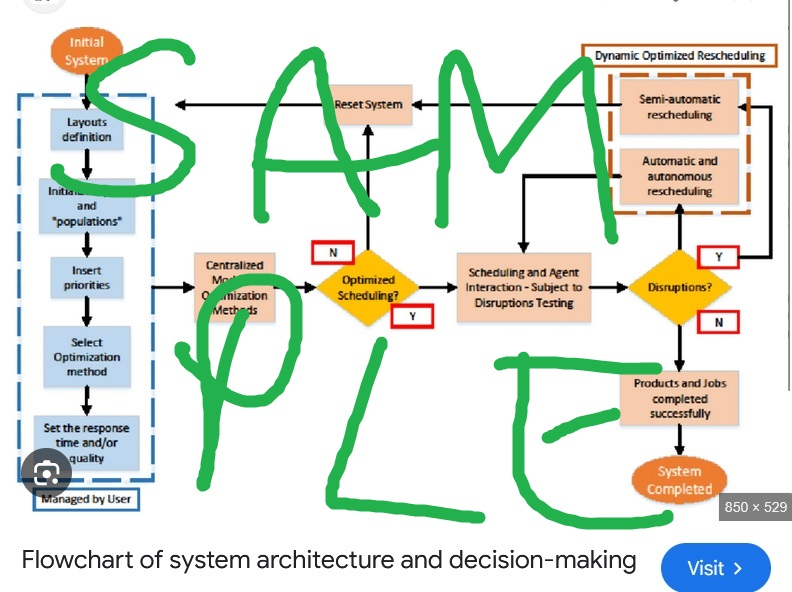
\includegraphics[width=0.6\textwidth]{figures/methodology/system_architecture.jpg}
    \caption{System Architecture Diagram}
    \label{fig:system-architecture5}
\end{figure}